\section{Method\textsuperscript{1}}
\begin{figure}[ht]
    \centering
    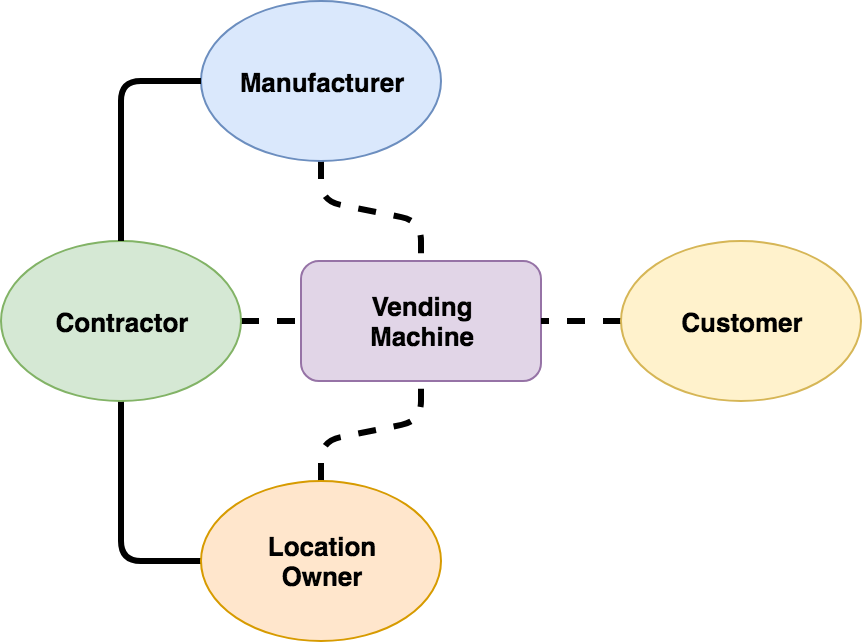
\includegraphics[width=0.4\textwidth]{assets/relations.png}
    \caption{Actors of the systems}
    \label{fig:relations}
\end{figure}
The typical business models for vending machines consists of multiple \textit{stakeholders} (see Figure \ref{fig:relations}), where at least a \textit{location owner} and a \textit{contractor} is involved. The contractor can operate independently or in a larger scale business model as shown in Figure \ref{fig:relations2}, in cooperation with the vending machine \textit{manufacturer}. The contractor is responsible for item refilling and maintenance of a vending machine whereby the location owner provides the physical space for a vending machine installation. Regardless of the business model scale, all actors share the profit, which requires a certain degree of mutual trust. For example, all stakeholders must trust the contractor's reports on the vending machine's revenues.
\begin{figure}[ht]
    \centering
    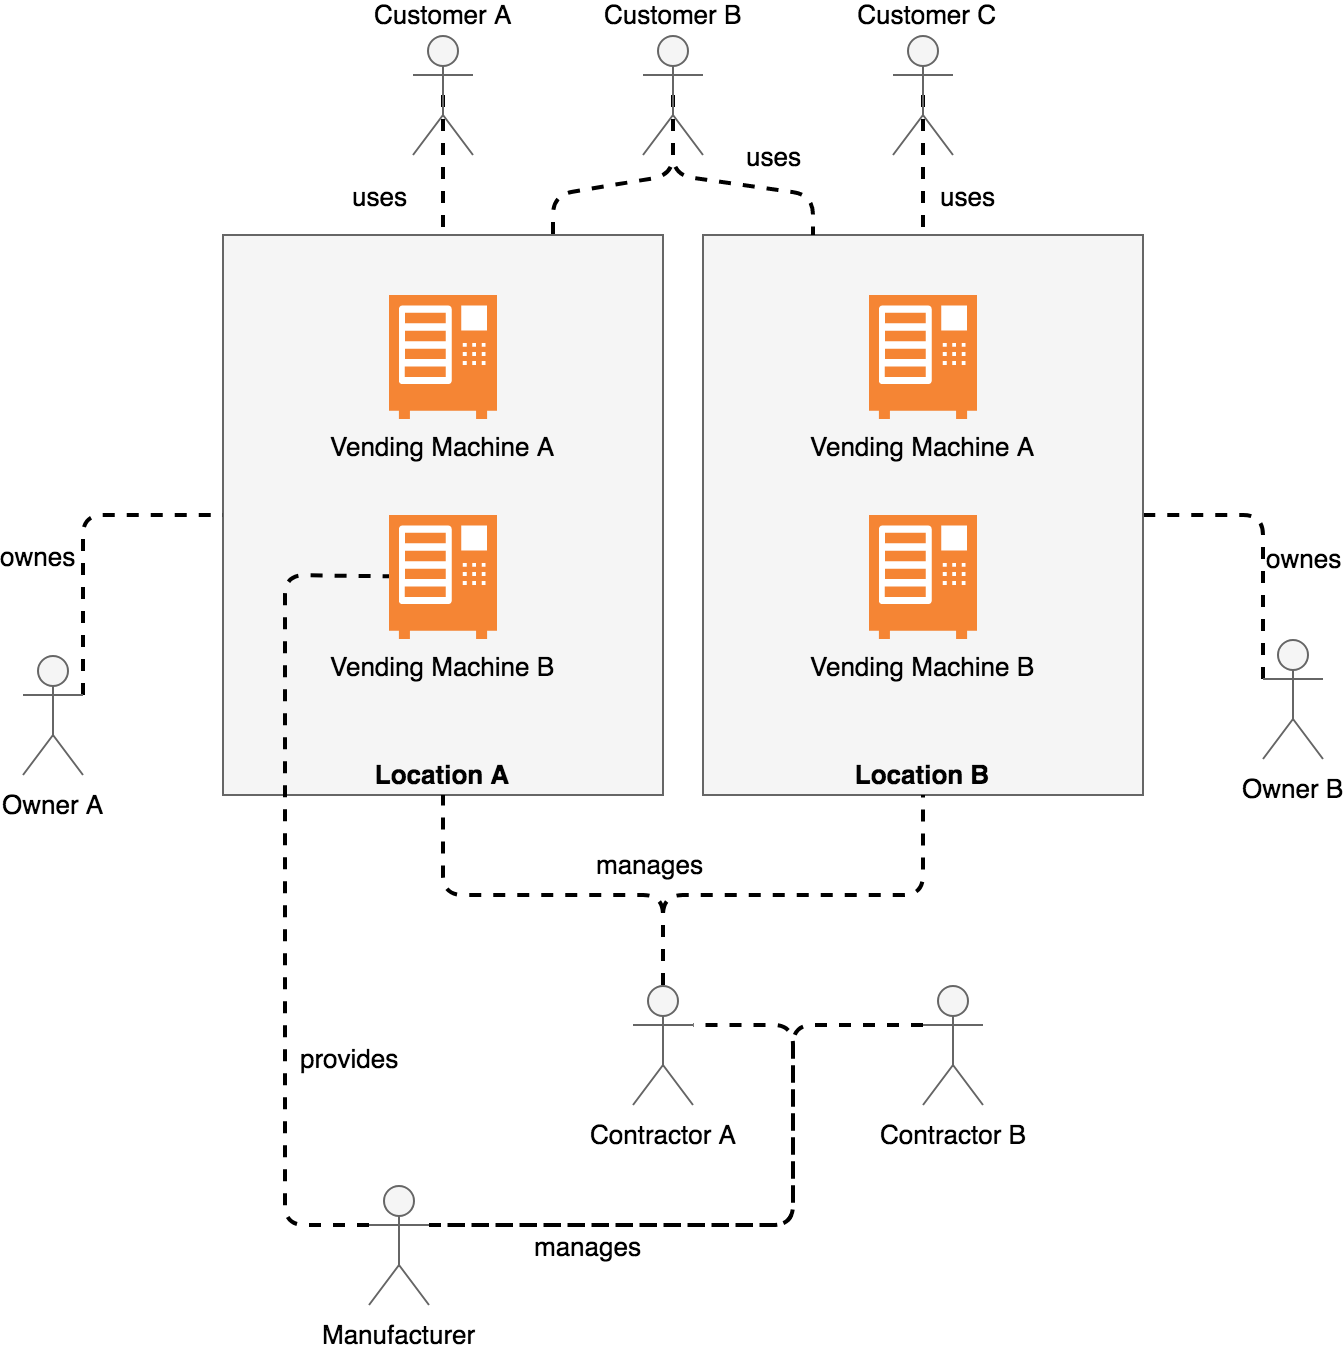
\includegraphics[width=0.49\textwidth]{assets/relations2.png}
    \caption{Relationships between the actors}
    \label{fig:relations2}
\end{figure}
A second view point is the \textit{customers} perspective, who prefers an effortless and quick electronic payment at the vending machine. The customer uses the vending machines on different locations but might be accustomed to use the same payment method on all locations. \\
For both view points, a blockchain technology can help to solve the described issues. Due to the distributed ledger technology, each stakeholder manages a copy of the ledger, which provides transparency in the system. At the same time, the blockchain technology forces all stakeholders to agree on the global state of the ledger to avoid manipulations of the ledger. These requirements can be summarized as the following. \\
\begin{itemize}
  \item quick, effortless payments for customers
  \item low payment processing time to avoiding queues in rush hours
  \item easy and intuitive use by customers
  \item comparable or better user experience for customers, compared to cash payment
  \item transparency for all actors
  \item no or low transactions fees for payment processing
  \item no costs for device management
  \item ability to integrate additional payment providers
\end{itemize}
The proposed system aims to implement a management architecture for pay-per-use business cases, especially for vending machines, with percentage-wise profit sharing, inventory management and payment processing, on a blockchain. A blockchain approach is being pursued to create a transparent, trusted environment for all stakeholders of the system, more precisely the manufacturer, the contractors and the location providers. From an user-experience oriented point of view, payment transaction speed should be comparable to familiar methods, like cash payment or EC payment, to incentivize acceptance and adoption. With most blockchain based solutions, this criterion is difficult to fulfill, while maintaining a secure transaction confirmation threshold. The nature of blockchain based solutions allows a high level of reliability and trust because of a redundant number of peers as an integral part of the consensus mechanism, which eliminates a single point of failure.

\subsection{Approach}

As described in the Background section, many blockchain technologies are already in active use and common cryptocurrencies like Bitcoin or Ethereum can rather easily be acquired through a myriad of specialized cryptocurrency exchanges. Though, the transaction confirmation time, easily taking a few minutes on most blockchain platforms, does not fulfill an essential requirement for our architecture. The unpredictable and highly fluctuating transaction fees, which we already recognized in the background section as a main obstacle, would hamper the adoption of the proposed system and render every advantage, the system provides for management of vending machines, insignificant. \\
Of all distributed ledger platforms discussed, only the Ethereum Platform and the Hyperledger Fabric Framework allow the implementation of business logic in smart contracts which is essential for transparency in this pursued triangular business model. But with Ethereum, not only the payment process itself would result in transaction fees, also every management operation that invokes the smart contract, for example updating prices of items, creates costs. As of this, the Hyperledger Fabric framework, with nearly instant transactions and no transaction fees, would be an ideal solution for implementation of the introduced architecture, but it lacks a native integrated cryptocurrency for monetary balance settlement, because of an enterprise oriented focus.

To develop a convincing solution, the proposed method uses a combination of both approaches, to achieve instant transactions and the usage of popular cryptocurrencies. For this, the business logic of the model described earlier in this chapter is implemented with the Hyperledger Fabric framework, which allows transparency and trust for all stakeholders involved. The business logic further maintains a balance for each customer, which can be redeemed on vending machines and recharged using popular cryptocurrencies. The customer is able to buy a product instantly at a vending machine and can make deposits to his account balance with various different payment providers, due to a modular approach. \\
Permissioned blockchains like Hyperledger Fabric require the authentication of each participant in the network. Therefore each stakeholder (see Figure \ref{fig:relations2}) and application component of the network (see Figure \ref{fig:systemarch}), uses x509 certificates for authentication. The certificate consist of a public and a private key and is used to sign every transaction, resulting from the interaction with the network, with the private key portion.

For the identification of the customer, we compared QR codes, NFC and Bluetooth technologies. Using a smartphone, the customer would be able to generate a unique QR code linked to his account and use it for identification at the vending machine. This approach would require a QR code reader for the recognition and a method to indicate a proper alignment between QR code reader and smartphone. We concluded that this concept is not ideal user-experience wise because of high probability of errors in the scanning process. \\
Perfectly suited to our use case, the range of Near Field Communication (NFC) is limited to close proximity between the user device and the NFC unit at the vending machine. Depending on the device manufacturer, smartphones support different standards and formats regarding NFC protocols. Apples iOS for instance, currently only supports tags in NFC Data Exchange Format \\ (NDEF) \cite{apple-nfc:online} and the API is not able to emulate NFC tags or more precisely, only supports reading of tags. The emulation of NFC tags is an essential aspect for identification of the user. In addition to the protocol restrictions of the iOS stack, the availability of NFC modules in smartphones further restricts this approach.\\
Because Bluetooth is supported in nearly all smartphones, we also evaluated an approach based on this technology. Apple iOS and Google Android both support the beacon Bluetooth profile, however the identification of individual users in a waiting queue might be problematic.

\subsection{System architecture and components}
\begin{figure}[ht]
\centering
  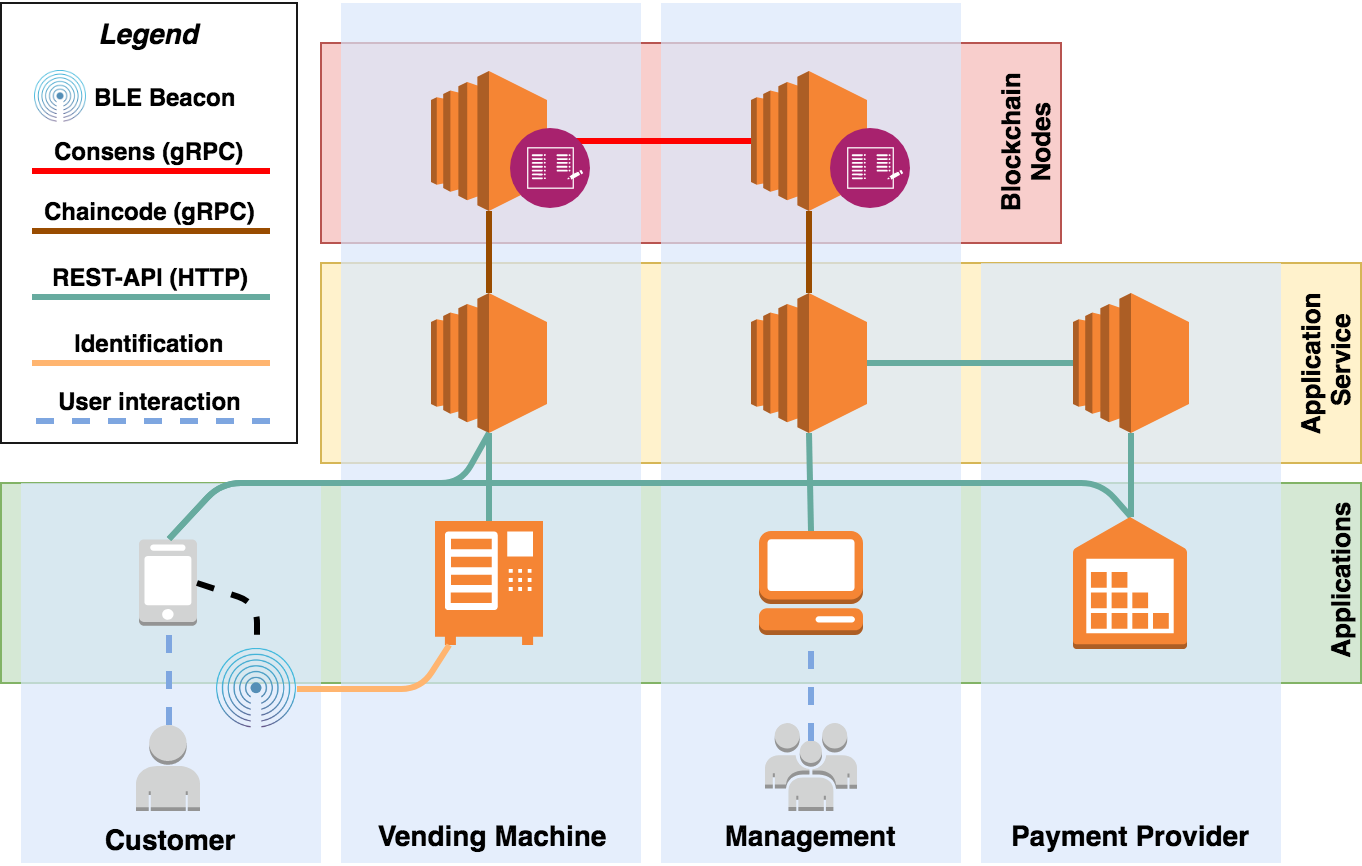
\includegraphics[width=0.5\textwidth]{assets/systemarch.png}
\caption{Architecture of the system components}
\label{fig:systemarch}
\end{figure}
Our proposed architecture is built on a layered structure of the components depicted in Figure \ref{fig:systemarch}, allowing a distributed deployment and a future functionality extension of the system through a loosely coupled design. \\
Because of the low availability of Near Field Communication (NFC) modules in smartphones and the intentionally restricted access to the lower layer of the NFC protocol in Apple devices, the proposed approach uses the Bluetooth beacon protocol for the identification of the customer at the vending machine. With the ongoing prevalence of NFC in smartphones and the programmatic access for third-party developers, user authentication at vending machines via NFC might get the preferred technique.\\
The system components are mainly developed using NodeJs and Typescript. The NodeJS ecosystem provides powerful tools and components for cross-platform projects, while allowing the reuse of common parts of the application between the different platforms like a mobile application, a web application or even embedded devices. In the following sections, we provide a description of the layers and components in detail.

\subsubsection{Blockchain nodes}
Each vending machine operates a blockchain node or \textit{peer} in Hyperledger Fabric terms, in order to increase protection against manipulation. For vending machines with a lower computational power, it is also possible to group several vending machines, based on the location or other criteria and use an edge device or even a cloud based service to operate the peer. 

Optionally, each stakeholder can also operate a peer with the full copy of the distributed ledger. Because multiple peers share the state of the blockchain, where all payments transactions get stored, no stakeholder is able to manipulate or forge earnings, which satisfies the requirement for profit-sharing business models. 

The logic of the business model is implemented in the chaincode of the Fabric framework and ensures that no chaincode invocation violates these rules. For instance the chaincode ensures that a customer is not able to purchase a product which exceeds the credits available on his account.

\subsubsection{Application service}
The application service layer consists of a REST service for the mobile application, vending machine and the management application described the next sections. The service is secured by the x509 certificate described earlier in this chapter and provides access to the network of Hyperledger Fabric peers. 

Depending on the payment provider, the application service layer also includes a service for the payment method which is responsible for the approval of a transactions, received from an external system or blockchain. It acts as a gateway between the proposed system and the external payment provider and deposits the transactions to the account of the customer as soon as they are approved. This decouples the transaction approval time described in the Section Background, from the actual payment process at the vending machine.

\subsubsection{Vending machine}
The vending machine dispenses goods such as food or drinks when a payment is received. Like described in the introduction of the chapter, the proposed method uses the Bluetooth Beacon protocol for identification of the customer. In this process, the customer selects the wanted product and is then requested to place the Beacon advertised by the mobile application on the smartphone to a specific area of the vending machine. The vending machine reads the account linked with the advertised beacon from the distributed ledger and requests to redeem the amount of the selected product. If the invocation of the redeem function in the chaincode succeeds, the requested good is dispensed.

\subsubsection{Mobile application}
\begin{figure}[ht]
\centering
  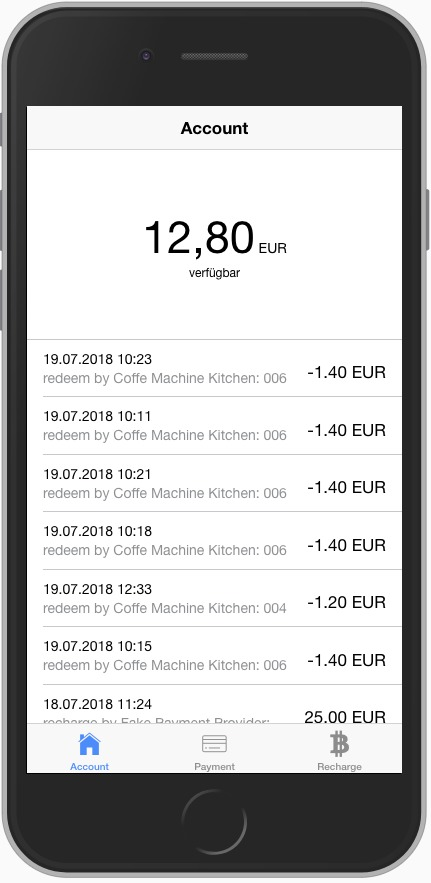
\includegraphics[width=0.45\textwidth]{assets/mobileapp.jpeg}
\caption{Account overview and transaction history}
\label{fig:mobile}
\end{figure}
Using the mobile application the customers is able to review the balance and the transaction history of his account (see Figure \ref{fig:mobile}). The transaction history includes the payouts from product purchases and deposits from payment providers. This provides the customer a transparent and verifiable insight into the account balance. 

For the identification, the customer must explicitly select the \textit{Payment} tab (see Figure \ref{fig:mobile}) in order to activate the advertisement of the Beacon. To minimize failures of accidentally advertised Beacons, the Beacon is disable when the another tab is selected or the application is closed. The advertised beacon contains the id of the account, which is then used by the vending machine to retrieve information about the customer.

To recharge credits to the customers account, the mobile application enables the customer to choose between different payment providers. Depending on the provider, the customer is redirected to the application of the provider or gets instructions to perform to complete the deposit. The payment provider service, described in the Section Application service, is triggered as soon the payment is completed.

\subsubsection{Management application}
\begin{figure}[ht]
\centering
  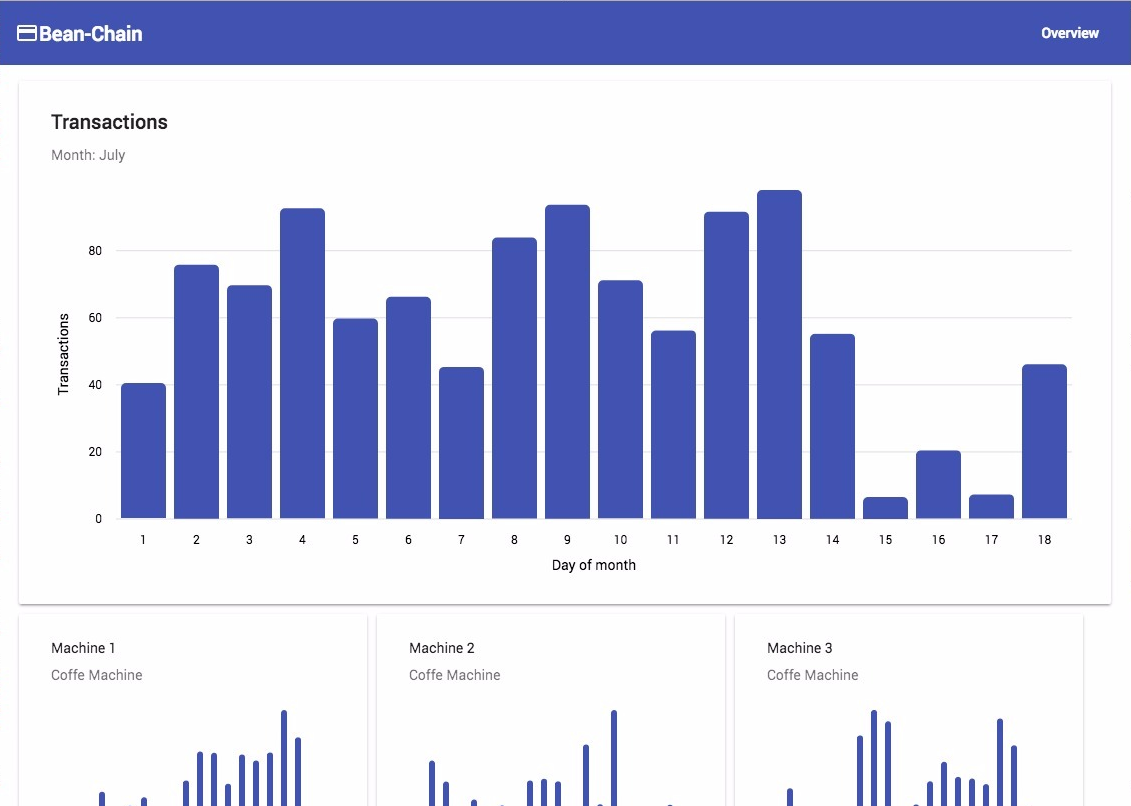
\includegraphics[width=0.49\textwidth]{assets/managment.png}
\caption{Management and analytics of vending machines}
\label{fig:management}
\end{figure}
The management application enables the stakeholders to get an overview of transactions linked to the vending machines manged by each stakeholder. The location owners can see all transactions regarding the vending machines of the locations. The contractors can manage all machines, which they maintain on different locations. The device manufactures have the highest level of visibility and can view  all the machines managed by their contractors. All stakeholder have the ability to make strategic decisions based on analytical insights provided by the management application. For instance, a contractor could decide based on the performance of a location to reallocate vending machines between locations. Further faulty vending machines can be detected by visually analyzing the transactions and identifying missing transactions.

\subsubsection{Payment provider}
The payment provider is the gateway between the distributed ledger of the Hyperledger Fabric framework and the payment provider. Any payment provider, whether decentralized or centralized, can be connected by implementing the application interface to the distributed ledger network. For this purpose, the presented method exposes a REST-API and provides authentication certificates for each payment provider. The implementation of the payment provider depends on the application interface of the provider. For instance an Ethereum based payment provider could leverage smart contracts to notify the distributed ledger on received payments. \\
The payment provider interface can also be used to implement a hardware based payment terminal to accept cash as a source for recharging the balance of a customer.